% Lecture Template for ME3050-001-002-Tristan Hill - Spring 2020
% Dynamics Modeling and Controls
% Frequency Response

% I am finally converting my stuff to BEAMER

% Document settings

%\documentclass{beamer}                  % for presentation ?
\documentclass[handout]{beamer}  % for handout ?
\usepackage{beamerthemesplit}
\usepackage{amsmath}
\usepackage{listings}
\usepackage{multicol}
\usepackage{framed}
\usepackage{amssymb}


\lstdefinestyle{myCustomMatlabStyle}{
  language=Matlab,
  numbers=left,
  stepnumber=1,
  numbersep=10pt,
  tabsize=4,
  showspaces=false,
  showstringspaces=false
}
\lstset{basicstyle=\ttfamily\tiny,style=myCustomMatlabStyle}
%lstset{language=MATLAB,basicstyle=\ttfamily\small,showstringspaces=false}



\beamertemplateballitem

\definecolor{TTUpurple}{rgb}{0.3098, 0.1607, 0.5176} % TTU Purple (primary)
\definecolor{TTUgold}{rgb}{1.0000, 0.8666, 0.0000} % TTU Gold (primary)

\setbeamercolor{palette primary}{bg=TTUpurple,fg=TTUgold}
\setbeamercolor{palette secondary}{bg=black,fg=TTUgold}
\setbeamercolor{palette tertiary}{bg=black,fg=TTUpurple}
\setbeamercolor{palette quaternary}{bg=TTUgold,fg=black}
\setbeamercolor{structure}{fg=TTUpurple} % itemize, enumerate, etc
\setbeamercolor{section in toc}{fg=TTUpurple} % TOC sections

%\DeclareSymbolFont{bbold}{U}{bbold}{m}{n}
%\DeclareSymbolFontAlphabet{\mathbbold}{bbold}

%\newcommand{\bbfamily}{\fontencoding{U}\fontfamily{bbold}\selectfont}
%\DeclareMathAlphabet{\mathbbold}{U}{bbold}{m}{n}

%\usefonttheme{professionalfonts}

\newcommand{\vspccc}{\vspace{6mm}\\} % large vertical space
\newcommand{\vspcc}{\vspace{4mm}\\}   % medium vertical space
\newcommand{\vspc}{\vspace{2mm}\\}     % small vertical space

\newcommand{\hspcccc}{\hspace{10mm}} % large horizontal space
\newcommand{\hspccc}{\hspace{6mm}} % large horizontal space
\newcommand{\hspcc}{\hspace{4mm}}   % medium horizontal space
\newcommand{\hspc}{\hspace{2mm}}     % small horizontal space


\newcommand{\LT}{\mathcal{L}} % lagrangian

\newcommand{\LNUM}{2 } %Lecture number 2

\newcommand{\secondtitle}{The Bode Diagram}% second line of the title of this presentation , aka the topic of this lecture

\title{Frequency Response - Lecture \LNUM}
\author{ME3050 - Dynamics Modeling and Controls} % original formatting from Mike Renfro, September 21, 2004

\date{April  19, 2020}

\begin{document}

\lstset{language=MATLAB,basicstyle=\ttfamily\small,showstringspaces=false}

% Title page1 
\frame{\titlepage \center\textbf{\secondtitle}\vspcc}


% Section 0: Outline
\frame{

\large \textbf{Lecture \LNUM - \secondtitle} \vspc

 \begin{itemize}


	\item Review Frequency Response\vspc % Section 1: 

	\item Amplitude ratio in Decibels\vspc % Section 2
	
	\item The Bode Diagram\vspcc %Section 2

	\item Frequency Response in MATLAB\vspcc % Section 3

\end{itemize}

}


%Section 1: Review Frequency Response
\section{Review Frequency Response}

\subsection{Harmonic Input Function}
\frame{
\frametitle{Harmonic Input Function}

\small 
The term {\bf frequency response} is used to describe a system's response to a periodic input. Frequency response analysis focuses on a system's response to {\it harmonic} input such as sines and cosines. The input (forcing) function is written below.\vspcc

\begin{framed}
\scalebox{1.25}{$f(t)=Asin\left(\omega t\right)$}\vspccc

\renewcommand{\arraystretch}{1.5}
\begin{tabular}{ccc}
Amplitude of the Input, & \scalebox{1}{$A$} & \scalebox{1}{$ (N)$} \\
Frequency of Input, &\scalebox{1}{$\omega$} &  \scalebox{1}{$(\frac{rad}{s})$}\\
\end{tabular}
\end{framed}

}

\subsection{First Order Frequency Response}
\frame{
\frametitle{First Order Frequency Response}


\small


The steady state response we derived is shown. Remember, after some amount of time passes, the transient term will disappear leaving just the sinusoidal terms. \vspc
\begin{framed}
\scalebox{1}{$y_{ss}\left(t\right)=A|T\left(j\omega\right)|sin\left(\omega t+\angle T\left(j\omega\right)\right)=MAsin\left(\omega t+\phi\right)$}\vspcc

The amplitude ratio and phase shift can be found from $T(j\omega)$. \vspcc

\scalebox{1}{$M(\omega)=|T(j\omega)|=\frac{1}{\sqrt{1+\tau^2\omega^2}}$}\vspc

\scalebox{1}{$\phi(\omega)=\angle T\left(j\omega\right)=-tan^{-1}\left(\omega\tau\right)$}\vspc
\end{framed}

}


\subsection{Graph of Frequency Response}
\frame{
\frametitle{Graph of Frequency Response}

\small

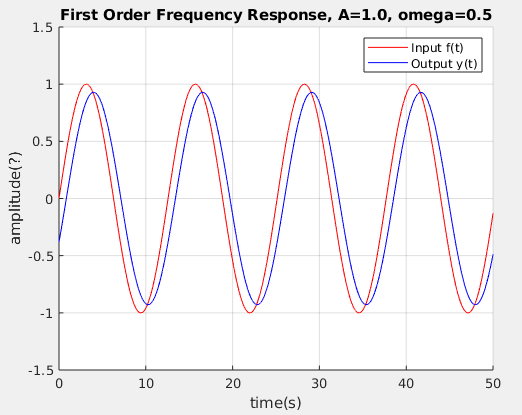
\includegraphics[scale=.275]{lecture1_fig6.png} \hspc 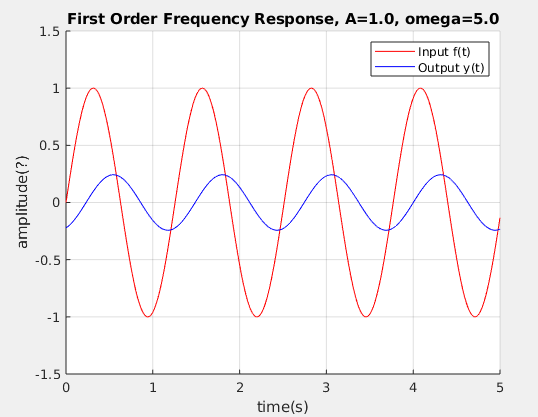
\includegraphics[scale=.275]{lecture1_fig5.png}  \vspc

The amplitude of the response is determined by the input frequency. \vspc

}


% section 2: The Bode Diagram

\section{The Bode Diagram}

\subsection{Dependence on Input Frequency}
\frame{
\frametitle{Dependence on Input Frequency}
\begin{multicols}{2}

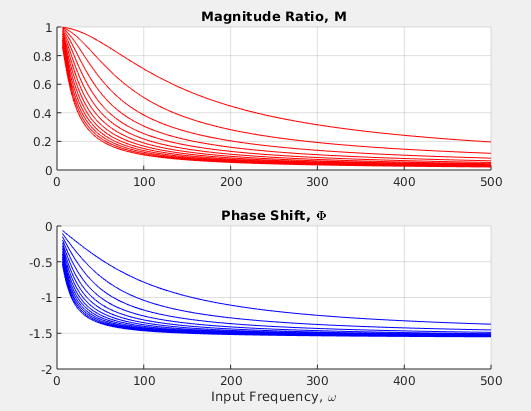
\includegraphics[scale=.27]{lecture2_fig2.png}

You can see that the amplitude ratio decreases as the input frequency increases. The individual curves represent systems with different time constants. 

\end{multicols}

}

\subsection{Review Properties of Logarithms}
\frame{
\frametitle{Review Properties of Logarithms}

\underline{Basic Properties of Logarithms:}\vspc
\renewcommand{\arraystretch}{1.5}
\begin{tabular}{cc}
Multiplication&\scalebox{1}{$log(pq)=log(p)+log(q) $} \\
Division&\scalebox{1}{$log(\frac{x}{y})=log(x)-log(y)$} \\
Power&\scalebox{1}{$log(x^n)=nlog(x)$}\\
\end{tabular}

\underline{Units of Decibels for Magnitude:}\vspc
\scalebox{1}{$m(dB)=10log(M^2)=20log(M)$ \hspccc convert back: \hspccc $M=10^{\frac{m(dB)}{20}}$}\vspc

\small
Decibel (dB), unit for expressing the ratio between two physical quantities, usually amounts of acoustic or electric power, or for measuring the relative loudness of sounds. One decibel (0.1 bel) equals 10 times the common logarithm of the power ratio. - Britannica.com

}



\subsection{Amplitude ratio on a Logarithmic Scale}
\frame{
\frametitle{Amplitude ratio on a Logarithmic Scale}


These relationships are more useful shown on a logarithmic scale. We can make use of the properties of logarithms in our analysis. \vspcc

\scalebox{1}{$m\left(dB\right)=20log\left(\frac{1}{\sqrt{1+\omega^2\tau^2}}\right)=20\left(log\left(1\right)-log\sqrt{1+\omega^2\tau^2}\right)$}\vspc
\scalebox{1}{$m\left(dB\right)=20log\left(1\right)-10log\left(1+\omega^2\tau^2\right)=-10log\left(1+\omega^2\tau^2\right)$}\vspc
\begin{framed}
\scalebox{1}{$m\left(dB\right)=-10log\left(1+\omega^2\tau^2\right)$}\vspc amplitude ratio in decibels
\end{framed}
}

\subsection{Amplitude ratio on a Logarithmic Scale}
\frame{
\frametitle{Amplitude ratio on a Logarithmic Scale}
\begin{multicols}{2}

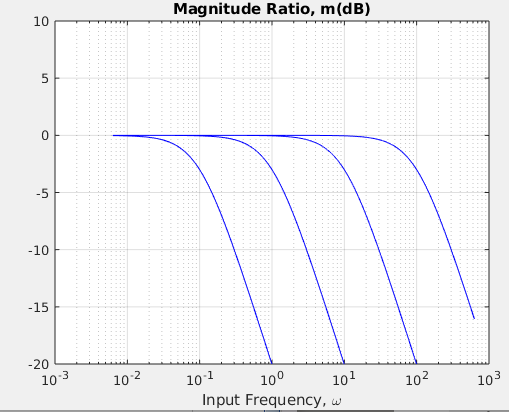
\includegraphics[scale=.30]{lecture2_fig7.png}
This is a Bode plot. It seems abstract but there is some very useful information shown.\vspc

  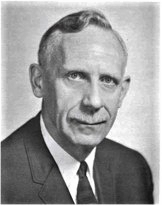
\includegraphics[scale=.4]{hendrikbode.png} \vspc Hendrik Bode (1905-1982) 

\end{multicols}
}

\section{Frequency Response in MATLAB}

\subsection{Bode Plot in MATLAB}
\frame[containsverbatim]{
\frametitle{Bode Plot in MATLAB}

MATLAB has a built it tool for making Bode plots.  
\begin{multicols}{2}
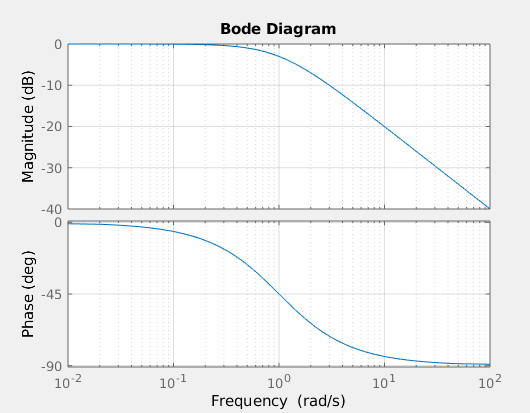
\includegraphics[scale=.25]{lecture2_fig9.png}

\begin{lstlisting}
figure(1)
sys=tf(1,[tau(3) 1])
bode(sys);grid on
\end{lstlisting}

\end{multicols}

So what? What can you do with a Bode diagram?

}

% references is not a section for now, for looks and it would be a waste of space
\frame{

\frametitle{References}

\begin{itemize}
	\item System Dynamics, Palm III, Third Edition - Chapter 9 - System Response in the Frequency Domain
\end{itemize}

}

\end{document}









 